
\documentclass{article}

% if you need to pass options to natbib, use, e.g.:
% \PassOptionsToPackage{numbers, compress}{natbib}
% before loading nips_2017
%
% to avoid loading the natbib package, add option nonatbib:
% \usepackage[nonatbib]{nips_2017}

\PassOptionsToPackage{numbers, sort}{natbib}
\usepackage[final]{nips_2017}
\bibliographystyle{unsrtnat}

\usepackage[final]{nips_2017}

% to compile a camera-ready version, add the [final] option, e.g.:
% \usepackage[final]{nips_2017}

\usepackage[utf8]{inputenc} % allow utf-8 input
\usepackage[T1]{fontenc}    % use 8-bit T1 fonts
\usepackage{hyperref}       % hyperlinks
\usepackage{url}            % simple URL typesetting
\usepackage{booktabs}       % professional-quality tables
\usepackage{amsfonts}       % blackboard math symbols
\usepackage{nicefrac}       % compact symbols for 1/2, etc.
\usepackage{microtype}      % microtypography

\usepackage{lipsum}
\usepackage{algpseudocode}

\usepackage{amssymb, amsmath}

\usepackage{graphicx}
\graphicspath{ {../R/} }

\title{Hierarchical Latent Space Models\\for Multiplex Social Network Analysis}

% The \author macro works with any number of authors. There are two
% commands used to separate the names and addresses of multiple
% authors: \And and \AND.
%
% Using \And between authors leaves it to LaTeX to determine where to
% break the lines. Using \AND forces a line break at that point. So,
% if LaTeX puts 3 of 4 authors names on the first line, and the last
% on the second line, try using \AND instead of \And before the third
% author name.

\author{
  Alex Martin Loewi \\
  \texttt{aloewi@cmu.edu}
  \And
  Francisco Ralston Fonseca\\
  \texttt{fralston@andrew.cmu.edu}
%  \And
%  Octavio Mesner\\
%  \texttt{omesner@cmu.edu}
  %% examples of more authors
  %% \And
  %% Coauthor \\
  %% Affiliation \\
  %% Address \\
  %% \texttt{email} \\
  %% \AND
  %% Coauthor \\
  %% Affiliation \\
  %% Address \\
  %% \texttt{email} \\
  %% \And
  %% Coauthor \\
  %% Affiliation \\
  %% Address \\
  %% \texttt{email} \\
  %% \And
  %% Coauthor \\
  %% Affiliation \\
  %% Address \\
  %% \texttt{email} \\
}

\begin{document}
% \nipsfinalcopy is no longer used

\maketitle

\begin{abstract}
An extension of the Latent Space Model is developed, for parsimoniously fitting multigraph data. The model finds embeddings for all of the graph layers in a way that makes them visually comparable, a difficult to achieve but important property for social network analysis and many other fields including medical diagnostics, and deep learning. The model is fit using a group LASSO penalty that both increases interpretability, and also allows for graph-wise dimensionality reduction of this complicated form of data. Results are demonstrated on a novel data set of eighty individuals from the staff of a charter school.
\end{abstract}

\section{Introduction}

\subsection{The Difficulty and Ubiquity of Multigraphs} %Curious Case of SNA}
%Social network analysis (SNA) is a complex, and inherently interdisciplinary field. It takes the already complex fields of psychology and sociology, and focuses on the most interdependent processes in these disciplines. This then creates systems so complicated that sophisticated statistical models are necessary to make any sense of them. While this complexity makes SNA an exciting intersection, effectively spanning these two disparate approaches is exceptionally difficult. As a result, while it attracts a great deal of attention, many important problems in SNA are under-studied, simply because of the small number of people who are trained to deal with both the substance, and methods, of the field.

Multigraphs, also called multiview networks, can be thought of as either a single graph with multiple edge types, or as multiple networks over the same set of nodes. Data of this kind is not uncommon, at either large or small scales. Twitter has Following relationships, as well as Retweets, and Likes, each of which can be thought of as simply one layer within the full relationship between two nodes. In small scales, surveys for networks very rarely ask about a single type of relationship, and many of the most famous network data sets have multiple relationships (such as Trust, Friendship, and Respect, in Samson's monk data). Despite the existence of data of this form for decades, its inherent difficulty has led to only a small number of models for it, all of which have important shortcomings for the practicing social network analyst.

% The models from statistics tend to ignore the problems of the practitioner, and the practitioners rarely have the training to develop their own methods.

\subsection{The Practical Difficulties of Multigraphs}
In particular, practitioners have two immediate problems when dealing with multigraphs, both of which are consequences of the inherent complexity of the data.

\subsubsection{Visualization}
The first problem is that multigraphs are too complex to easily visualize, and visualization has always been a cornerstone of network analysis. In particular, the difficulty comes in comparing the many layers of data (i.e. the graphs formed by the different edge types). To be expressive, a graph layout needs to be flexible in how it places nodes -- however in order to be comparable, two layouts need to place nodes in relatively similar places. A useful multigraph model would be able to tune explicitly between these two extremes of flexibility, and comparability.

\subsubsection{Dimensionality}
The second problem is that multigraphs may be unnecessarily complex. Empirically, there are often high degrees of correlation between the layers in a multigraph, and the smaller the number of graphs, the easier analysis becomes. These two observations combine to suggest another useful property of a new model -- the ability to remove redundant layers.


\subsection{Previous Work}

% SOME OF THESE CITATIONS AREN'T RIGHT -- don't have the original lasso paper, may be the major issue. Also, these emphasize the coordinate descent, which aren't a part of the paper right now

Our model combines several methods that have proven to be exceptionally valuable -- Latent Space Models, \cite{Hoff2002}, the LASSO estimator, \cite{Friedman2008}, and in particular the group LASSO \cite{Yuan2008}. The substantial amount of work that has been done on them all provides many different possible approaches to designing, and fitting, our own model. Efficient optimization procedures, often employing coordinate or block-coordinate optimization, exist for fitting the LASSO to linear models, \cite{Friedman2008}, to generalized linear models \cite{Friedman2010}, with the element-wise, group, and combined, sparse group LASSO, \cite{Vincent, Qin, Wu2008}, and more.

When it comes to LSMs for multigraphs, this year already, two different papers have been published that take this general appraoch -- however, our approach has important advantages over both of them. One paper takes the extreme of modeling the multigraph as a single object, which only makes visualization more difficult \cite{gollini-2016}. The other treats each layer as independent, and allows correlations between them. While a highly intuitive idea, this does not solve the comparability problem, or that of dimensionality reduction \cite{salter-townshend2017}. Furthermore, allowing correlations between layers means that an edge may exist either because its positions are close, or because the positions in a correlated layer are close. This ambiguity, while expressive, may lead to a problem with identifiability that would be a serious issue for the interpretation of modeled social systems. %may lead to an ambiguity that would not be desirable for interpretation.

\section{The Model}
\subsection{Problem Statement}
Motivated by these problems, we propose a model with the following three objectives:

\begin{enumerate}
\item Use current methods from statistical SNA to model multigraphs
\item Model the layers of the multigraph in a way that can tune between comparability and expressiveness
\item Allow the model to remove redundant layers
\end{enumerate}

A model with all of these qualities, which we term the Hierarchical Latent Space Model, can be described in the following way:

\subsection{The Likelihood Function}
Using the canonical Latent Space Model \cite{Hoff2002} as a starting point, we model a set of conditionally independent binary dyads. 

The existence of each of these dyads is a function of an intercept, a set of covariates (omitted here for clarity), and the distance between the latent ``position'' variables $z$ of the two nodes in the dyad. The goal of the model will be to estimate these positions. An optimal set of variables would place positions close together for nodes with an observed edge, and vice versa.

\[
\eta_{ijk} = \alpha_k - \|z_{ik} - z_{jk}\|_2^2 %=  \alpha_k - \|b_i + \epsilon_{ik} - b_j - \epsilon_{jk}\|^2
\]

The indices $i$ and $j$ are over the nodes; the index $k$ refers to the different layers in the multigraph. Because the edges are binary, we use the inverse logit $\sigma$ to transform $\eta$, but it should be observed that for real-valued edges, other link functions could be easily substituted.

\[
\sigma(\eta_{ijk}) = \frac{1}{1+\exp(-\eta_{ijk})} \in [0, 1]
\]

All together, the unpenalized likelihood of the HLSM thus takes the form of a binomial:

\begin{align*}
  L &= \prod_k \prod_{i}\prod_{j<i} \sigma(\eta_{ijk})^{y_{ijk}}(1-\sigma(\eta_{ijk}))^{1-y_{ijk}}
\end{align*}

and the log likelihood is

\begin{align*}
  \ell 	%&= \sum_k \sum_{i} \sum_{j < i} {y_{ijk}} \ln \sigma(\eta_{ijk}) + (1-y_{ijk})\ln(1- \sigma(\eta_{ijk})) \\
  	%&= \sum_k \sum_{i} \sum_{j < i} - {y_{ijk}} \ln (1+\exp(-\eta_{ijk})) + (1-y_{ijk})\ln\left (\frac{\exp(-\eta_{ijk})}{1+\exp(-\eta_{ijk})}\right) \\
  	%&= \sum_k \sum_{i} \sum_{j < i} - {y_{ijk}} \ln (1+\exp(-\eta_{ijk})) + (1-y_{ijk})[-\eta_{ijk} - \ln (1+\exp(-\eta_{ijk}))] \\
  	%&=\sum_k \sum_{i} \sum_{j < i} - {y_{ijk}} \ln (1+\exp(-\eta_{ijk})) -\eta_{ijk} - \ln (1+\exp(-\eta_{ijk})) + y_{ijk} \eta_{ijk} + y_{ijk}\ln (1+\exp(-\eta_{ijk}))] \\
 	& = \sum_k \sum_{i} \sum_{j < i} (y_{ijk}-1)\eta_{ijk} - \ln (1+\exp(-\eta_{ijk}))
\end{align*}

\subsection{Regularization}

While the notation $z$ for the latent variables is consistent with the literature, and somewhat more intuitive, our contribution comes from a reparameterization of the model, where

\[
z_{ik} = b_i + \epsilon_{ik}
\]

Our model starts with a ``base'' position $b_i$ for each node, which is the hierarchical layer in the model. It then adds a layer-specific perturbation $\epsilon_{ik}$. The behavior of the model then depends entirely on the regularization placed on the $\epsilon$'s. When there is none, each layer is fit independently. When there is an arbitrarily large amount, the perturbations are all driven to zero, and all $k$ layers are represented identically by the base parameters $b$. With intermediate values, the user can find the point between these two extremes that allows for the graphs to be distinct, but also renders them sufficiently similar to be comparable, by not allowing the perturbations to stray too far from their shared base position.

Furthermore, with the use of a group lasso penalty that groups together all of the perturbations within a single layer $k$, the model will perform graph-wise dimensionality reduction, by setting a redundant layer equal to the base layer. This is far more valuable to the practitioner than an element-wise sparse solution, which would still require them to consider all of the layers in their multigraph. %This leads to the following penalized negative log likelihood, that we will attempt to optimize: 


%This parameterization takes an explicit mid-point between the two most recently published papers on this problem. One fits the layers independently, and allows correlations between them \cite{salter-townshend2013}; another  treats all of the layers simultaneously, as part of a single complex object \cite{gollini-2017}. Our model allows not only for similar behaviors to both of these extremes, but additionally allows the user to tune between them manually.

%\begin{align*}
% 	\ell = - \sum_k \sum_{i} \sum_{j < i} (y_{ijk}-1)\eta_{ijk} + \ln (1+\exp(-\eta_{ijk})) + \lambda \sum_k \|\epsilon_k\|_2
%\end{align*}

%\subsection{Derivations}


\section{Fitting}
\subsection{The Optimization Problem}

Together these two elements form our optimization problem, which is to minimize the sum of the negative log likelihood and a penalty on the deviations $\epsilon_{ik}$. We tested two approaches with respect to the penalty on the deviations $\epsilon_{ik}$. 

In the first model, we used an element-wise lasso, by penalizing the norm of each deviation $\epsilon_{ik}$. This can be seen in by Equation \ref{eq:lasso}. It is important to note that the latent parameters are all two-dimensional, to allow for visualization. Consequently even with this element-wise approach, the group-lasso approach and the L2 penalty is necessary, following \cite{Yuan2008}. However the grouping is only over the two dimensions of the individual parameter.  

\begin{align} \label{eq:lasso}
%\min_{\epsilon, b} \sum_k \sum_{i} \sum_{j < i} [ (1 - y_{ijk})\eta_{ijk} +  \ln (1+\exp(\eta_{ijk})) ] 
\min_{b, \epsilon} -\ell(b, \epsilon) + \lambda \sum_i\sum_{k} \| \epsilon_{ik}\|_2
\end{align}

In the second approach, we used a group lasso penalty that is over all of the perturbations $\epsilon_k$ within each layer $k$, instead of on each individual deviation $\epsilon_{ik}$. This encourages sparsity over the layers, meaning an entire graph might be zeroed out (expressed as just the base layer). This approach is illustrated in Equation \ref{eq:group_lasso}.

\begin{align} \label{eq:group_lasso}
%\min_{\epsilon, b} \sum_k \sum_{i} \sum_{j < i} [ (1 - y_{ijk})\eta_{ijk} +  \ln (1+\exp(\eta_{ijk})) ] 
\min_{b, \epsilon} -\ell(b, \epsilon) + \lambda \sum_k \| \epsilon_{k}\|_2
\end{align}



Because neither of these objective functions is differentiable, we use proximal gradient descent in fitting the model. %If the gradients for the ML function derived above are correct, we can directly use the code we implemented in HW3 (problem 4) to implement the proximal operator for this problem.

\subsection{Derivation of the Gradients}

%We define our decision variables as: $\{b_i\}$ $\forall~i$ and $\{\epsilon_{ik}\}$ $\forall~i,k$.

Then, the gradients of the $\eta_{ijk}$ are:

\[
\frac{\partial \eta_{ijk}}{\partial b_{i}} =  - 2(b_i + \epsilon_{ik} - b_j - \epsilon_{jk})
\]

\[
\frac{\partial \eta_{ijk}}{\partial b_{j}} = 2(b_i + \epsilon_{ik} - b_j - \epsilon_{jk})
\]

\[
\frac{\partial \eta_{ijk}}{\partial \epsilon_{ik}} = - 2(b_i + \epsilon_{ik} - b_j - \epsilon_{jk})
\]

\[
\frac{\partial \eta_{ijk}}{\partial \epsilon_{jk}} = 2(b_i + \epsilon_{ik} - b_j - \epsilon_{jk})
\]

\begin{align*}
\frac{\partial \ell}{\partial b_{m}} & =  \sum_k \sum_{i}  \sum_{j<i} (y_{ijk} -1)\frac{\partial \eta_{ijk}}{\partial b_{m}} - \frac{\partial \ln (1+\exp(-\eta_{ijk}))}{\partial b_{m}} \\
& =  \sum_k\left[ \sum_{j<m} (y_{mjk} -1)\frac{\partial \eta_{mjk}}{\partial b_{m}} - \frac{\partial \ln (1+\exp(-\eta_{mjk}))}{\partial b_{m}} +  \sum_{i > m} (y_{imk} -1)\frac{\partial \eta_{imk}}{\partial b_{m}} - \frac{\partial \ln (1+\exp(-\eta_{imk}))}{\partial b_{m}} \right] \\
%
& =  \sum_k\bigg[ -2 \sum_{j<m} \left[(y_{mjk} -1)(b_m + \epsilon_{mk} - b_j + \epsilon_{jk}) + \frac{\exp(-\eta_{mjk})}{1+\exp(-\eta_{mjk})}(b_m + \epsilon_{mk} - b_j - \epsilon_{jk}) \right] \\
& \quad\quad\quad +  2 \sum_{i > m} \left[(y_{imk} -1)(b_i + \epsilon_{ik} - b_m - \epsilon_{mk}) +\frac{\exp(-\eta_{ijk})}{1+\exp(-\eta_{mjk})}(b_i + \epsilon_{ik} - b_m - \epsilon_{mk}) \right] \bigg] \\
& =  2 \sum_k\bigg[ - \sum_{j<m} \left(y_{mjk} -1 + \frac{\exp(-\eta_{mjk})}{1+\exp(-\eta_{mjk})}\right)(z_{mk} - z_{jk})\\
& \quad\quad\quad\quad +  \sum_{i > m} \left(y_{imk} -1 + \frac{\exp(-\eta_{ijk})}{1+\exp(-\eta_{mjk})}\right)(z_{ik} - z_{mk}) \bigg] \\
%
\end{align*}

\begin{align*}
\frac{\partial \ell}{\partial \epsilon_{mk}} & = 2 \bigg[ - \sum_{j<m} \left(y_{mjk} -1 + \frac{\exp(-\eta_{mjk})}{1+\exp(-\eta_{mjk})}\right)(z_{mk} - z_{jk})\\
& \quad\quad +  \sum_{i > m} \left(y_{imk} -1 + \frac{\exp(-\eta_{ijk})}{1+\exp(-\eta_{mjk})}\right)(z_{ik} - z_{mk}) \bigg]
\end{align*}

\subsection{The Proximal Operator}

% \subsubsection{Group lasso}

The proximal operator for the penalty term using the L2 norm is: %\footnotemark~ is:

% \footnotetext{Using the results from Homework 3}

\[
\text{prox}_{\|.\|, \lambda t}(\epsilon_{k}) = 
\begin{cases}
\frac{\|\epsilon_{k}\| - \lambda t}{\|\epsilon_{k}\|}\epsilon_{k}, & \|\epsilon_{k}\| \ge \lambda t \\
0, & \|\epsilon_{k}\| < \lambda t
\end{cases}
\]

\[
\text{prox}_{\|.\|, \lambda t}(b_i) = b_i
\]

Therefore, let $\beta$ be the vector with all parameters $\epsilon$ and $b$. The Proximal Gradient Descent method in this case is:

\[
\beta^{+} = \text{prox}_{\|.\|, \lambda t}(\beta - t \nabla \ell(\beta))
\]

%\subsubsection{Standard lasso}
%
%The proximal operator for the penalty term using the L1 norm is:
%
%\[
%\text{prox}_{\|.\|_1, \lambda t}(\epsilon_{i, k}) = \text{sign}(\epsilon_{i, k})\max{(\epsilon_{i, k} - \lambda t, 0)}
%\]
%
%\[
%\text{prox}_{\|.\|_1, \lambda t}(b_i) = b_i
%\]
%
%Therefore, let $\beta$ be the vector with all parameters $\epsilon$ and $b$. The Proximal Gradient Descent method in this case is:
%
%\[
%\beta^{+} = \text{prox}_{\|.\|_1, t}(\beta - t \nabla \ell(\beta))
%\]


\subsection{Non-Convexity and Initialization}

The original Latent Space Model is known to be non-convex in the latent positions $z$ \cite{Hoff2002}, and our model is no different. This issue is typically approached by using MCMC samplers \cite{Hoff2002, salter-townshend2017} which are capable of exploring non-convex spaces, however using them on this problem proved not only to take far more time, but also to have substantially worse results. We focus our discussion on the convex approaches used.

As we use methods designed for convex problems, we start by using a careful initialization of our procedure. This attempts to begin the algorithm close to a global minimum of the objective, so that when we do descend the likelihood, we reduce our chances of being caught in a poor local minimum. This initialization was composed of several steps.

\\
\begin{enumerate}
\item Create a proposal `base' graph from $\hat{y}_{ij} =\sum_k y_{ijk} > 0$
\item Fit a separate single-graph latent space model to each layer (including the base layer)
\item Transform the layer estimates to minimize their distance from the base estimate
\end{enumerate}

The third step in this procedure was initially done with a Procrustes transform \cite{Hoff2002}, as is used in Bayesian estimation of Latent Space Models. This transform is used because proposal graphs in a sampling procedure can produce a graph with many different unimportant variations, as the likelihood is invariant to translation, rotation, scaling, and flipping. The Procrustes transform is thus used to remove these transformations, while keeping the variations that are of importance to the likelihood. However this transform minimizes the overall distance between \textit{all} pairs of points in two shapes, and in this problem, we require something slightly different. The goal here is to minimize only distances between positions that correspond to the same node -- this is the property that minimizes the $\epsilon$'s, and makes the embeddings comparable.

To solve this problem we propose the Anticrustean transformation. A closed form solution, should one exist, was not derived, but a simple implementation combines line searches over the several classes of transforms to which the likelihood is invariant. Together, these steps produce a good initial estimate of all of the models parameters, which are used as starting points in the proximal gradient procedure. 

%\begin{algorithmic}
%\If {$i\geq maxval$}
%    \State $i\gets 0$
%\Else
%    \If {$i+k\leq maxval$}
%        \State $i\gets i+k$
%    \EndIf
%\EndIf
%\end{algorithmic}

\section{Results}

To test our model, we first simulate a toy data set consisting of a multigraph with $N=20$ vertices and $K=2$ layers, followed by the real and novel data set that motivated this technique. We initialize our optimization problem using the initialization procedure described in the previous section. We then run $3000$ iterations of the proximal gradient algorithm. Figures \ref{fig:obj_lasso} and \ref{fig:obj_group} show the improvement in the objective function value over the 3000 iterations for, respectively, the element-wise lasso and the layer-wise lasso approaches using different values for $\lambda$. We can observe that the function values appear to converge to a local minimum. In both approaches we used a fixed step size $t=10^{-3}$ in the proximal gradient algorithms.


\begin{figure}[h!]
   \centering
   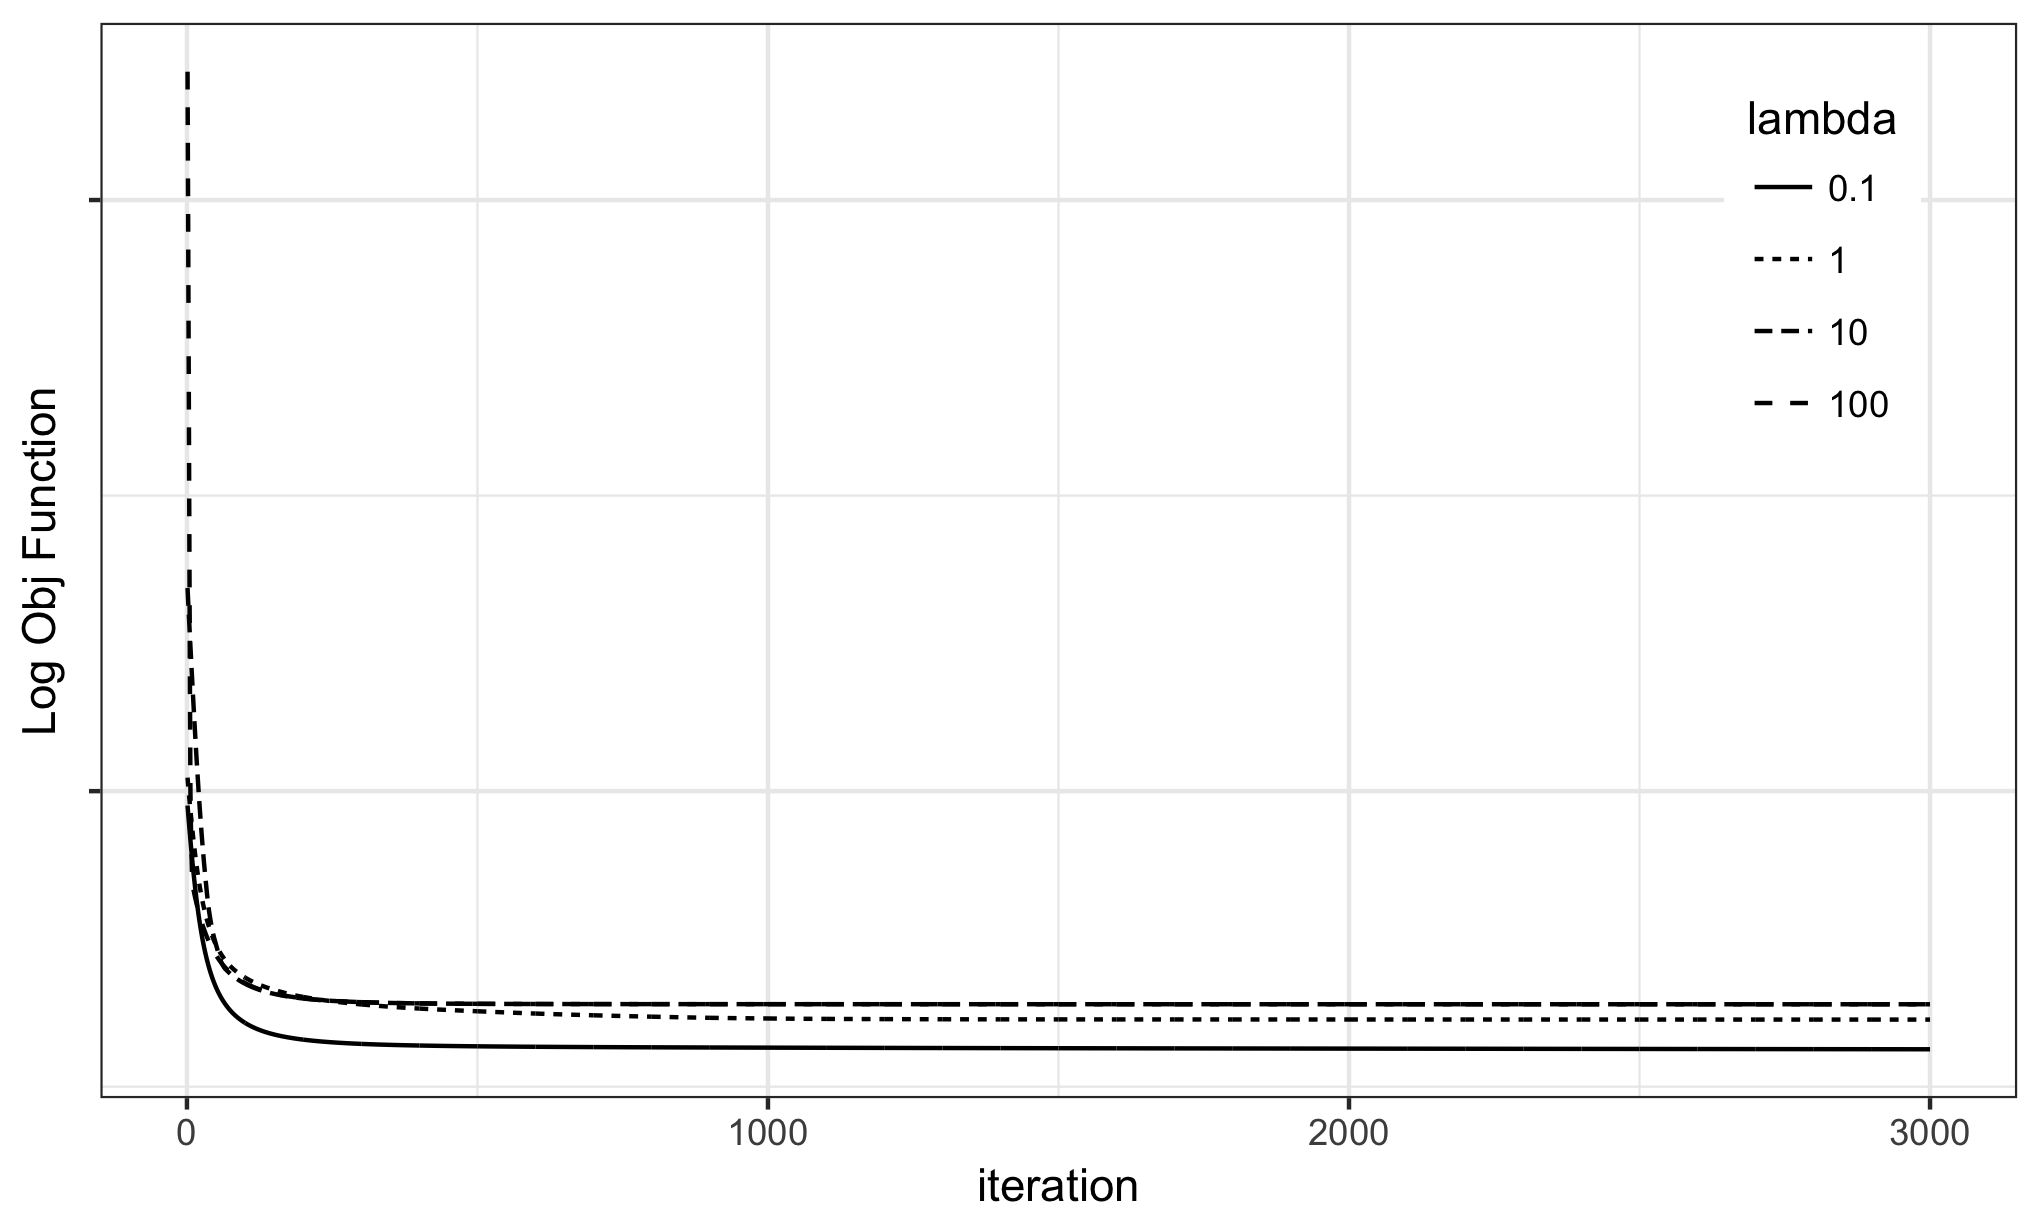
\includegraphics[width=0.4\textwidth]{plot_objective_individual} % requires the graphicx package
   \caption{Value of the objective function for different values of $\lambda$ in the standard lasso approach. We ran 3000 iterations of the proximal gradient descent algorithm.}
   \label{fig:obj_lasso}
\end{figure}

\begin{figure}[h!]
   \centering
   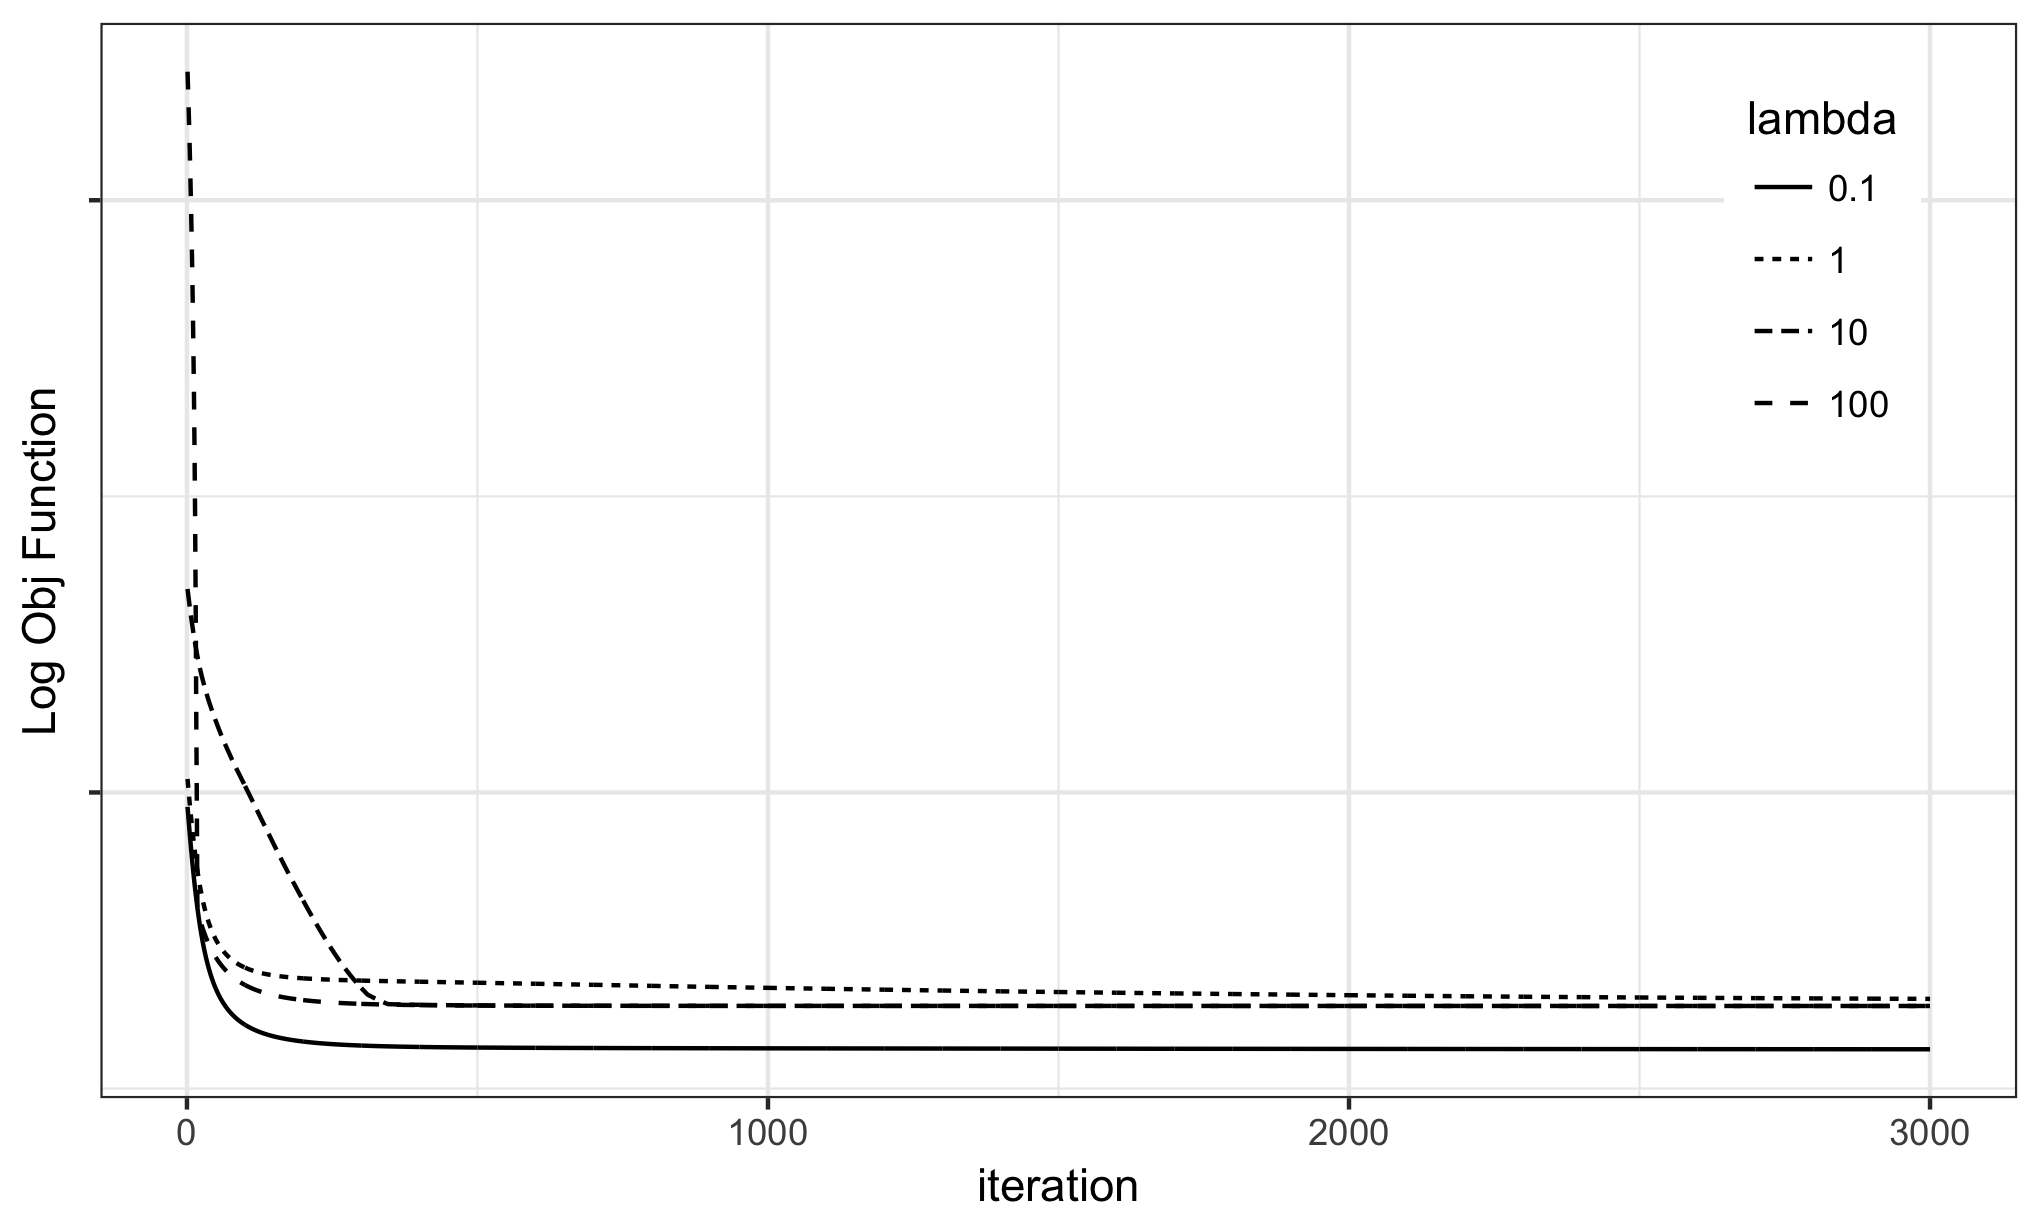
\includegraphics[width=0.4\textwidth]{plot_objective_group} % requires the graphicx package
   \caption{Value of the objective function for different values of $\lambda$ in the group lasso approach. We ran 3000 iterations of the proximal gradient descent algorithm.}
   \label{fig:obj_group}
\end{figure}

Figures \ref{fig:pos_lasso} and \ref{fig:pos_group} compare the optimal positions found by each of the models with the initial one. Black points represent the base positions $b_i$ and the red and green points (and lines) represent the two different layers of the graph. We can observe that as we increase the value of $\lambda$ deviations are more penalized and the optimal solution tends to be one where all layers collapse to a single graph. Additionally, we can also compare the resulting optimal positions between the two approached (standard lasso and group lasso). For $\lambda=1$ the two layers are significantly more distinct than the ones in the standard lasso case.

\begin{figure}[h!]
   \centering
   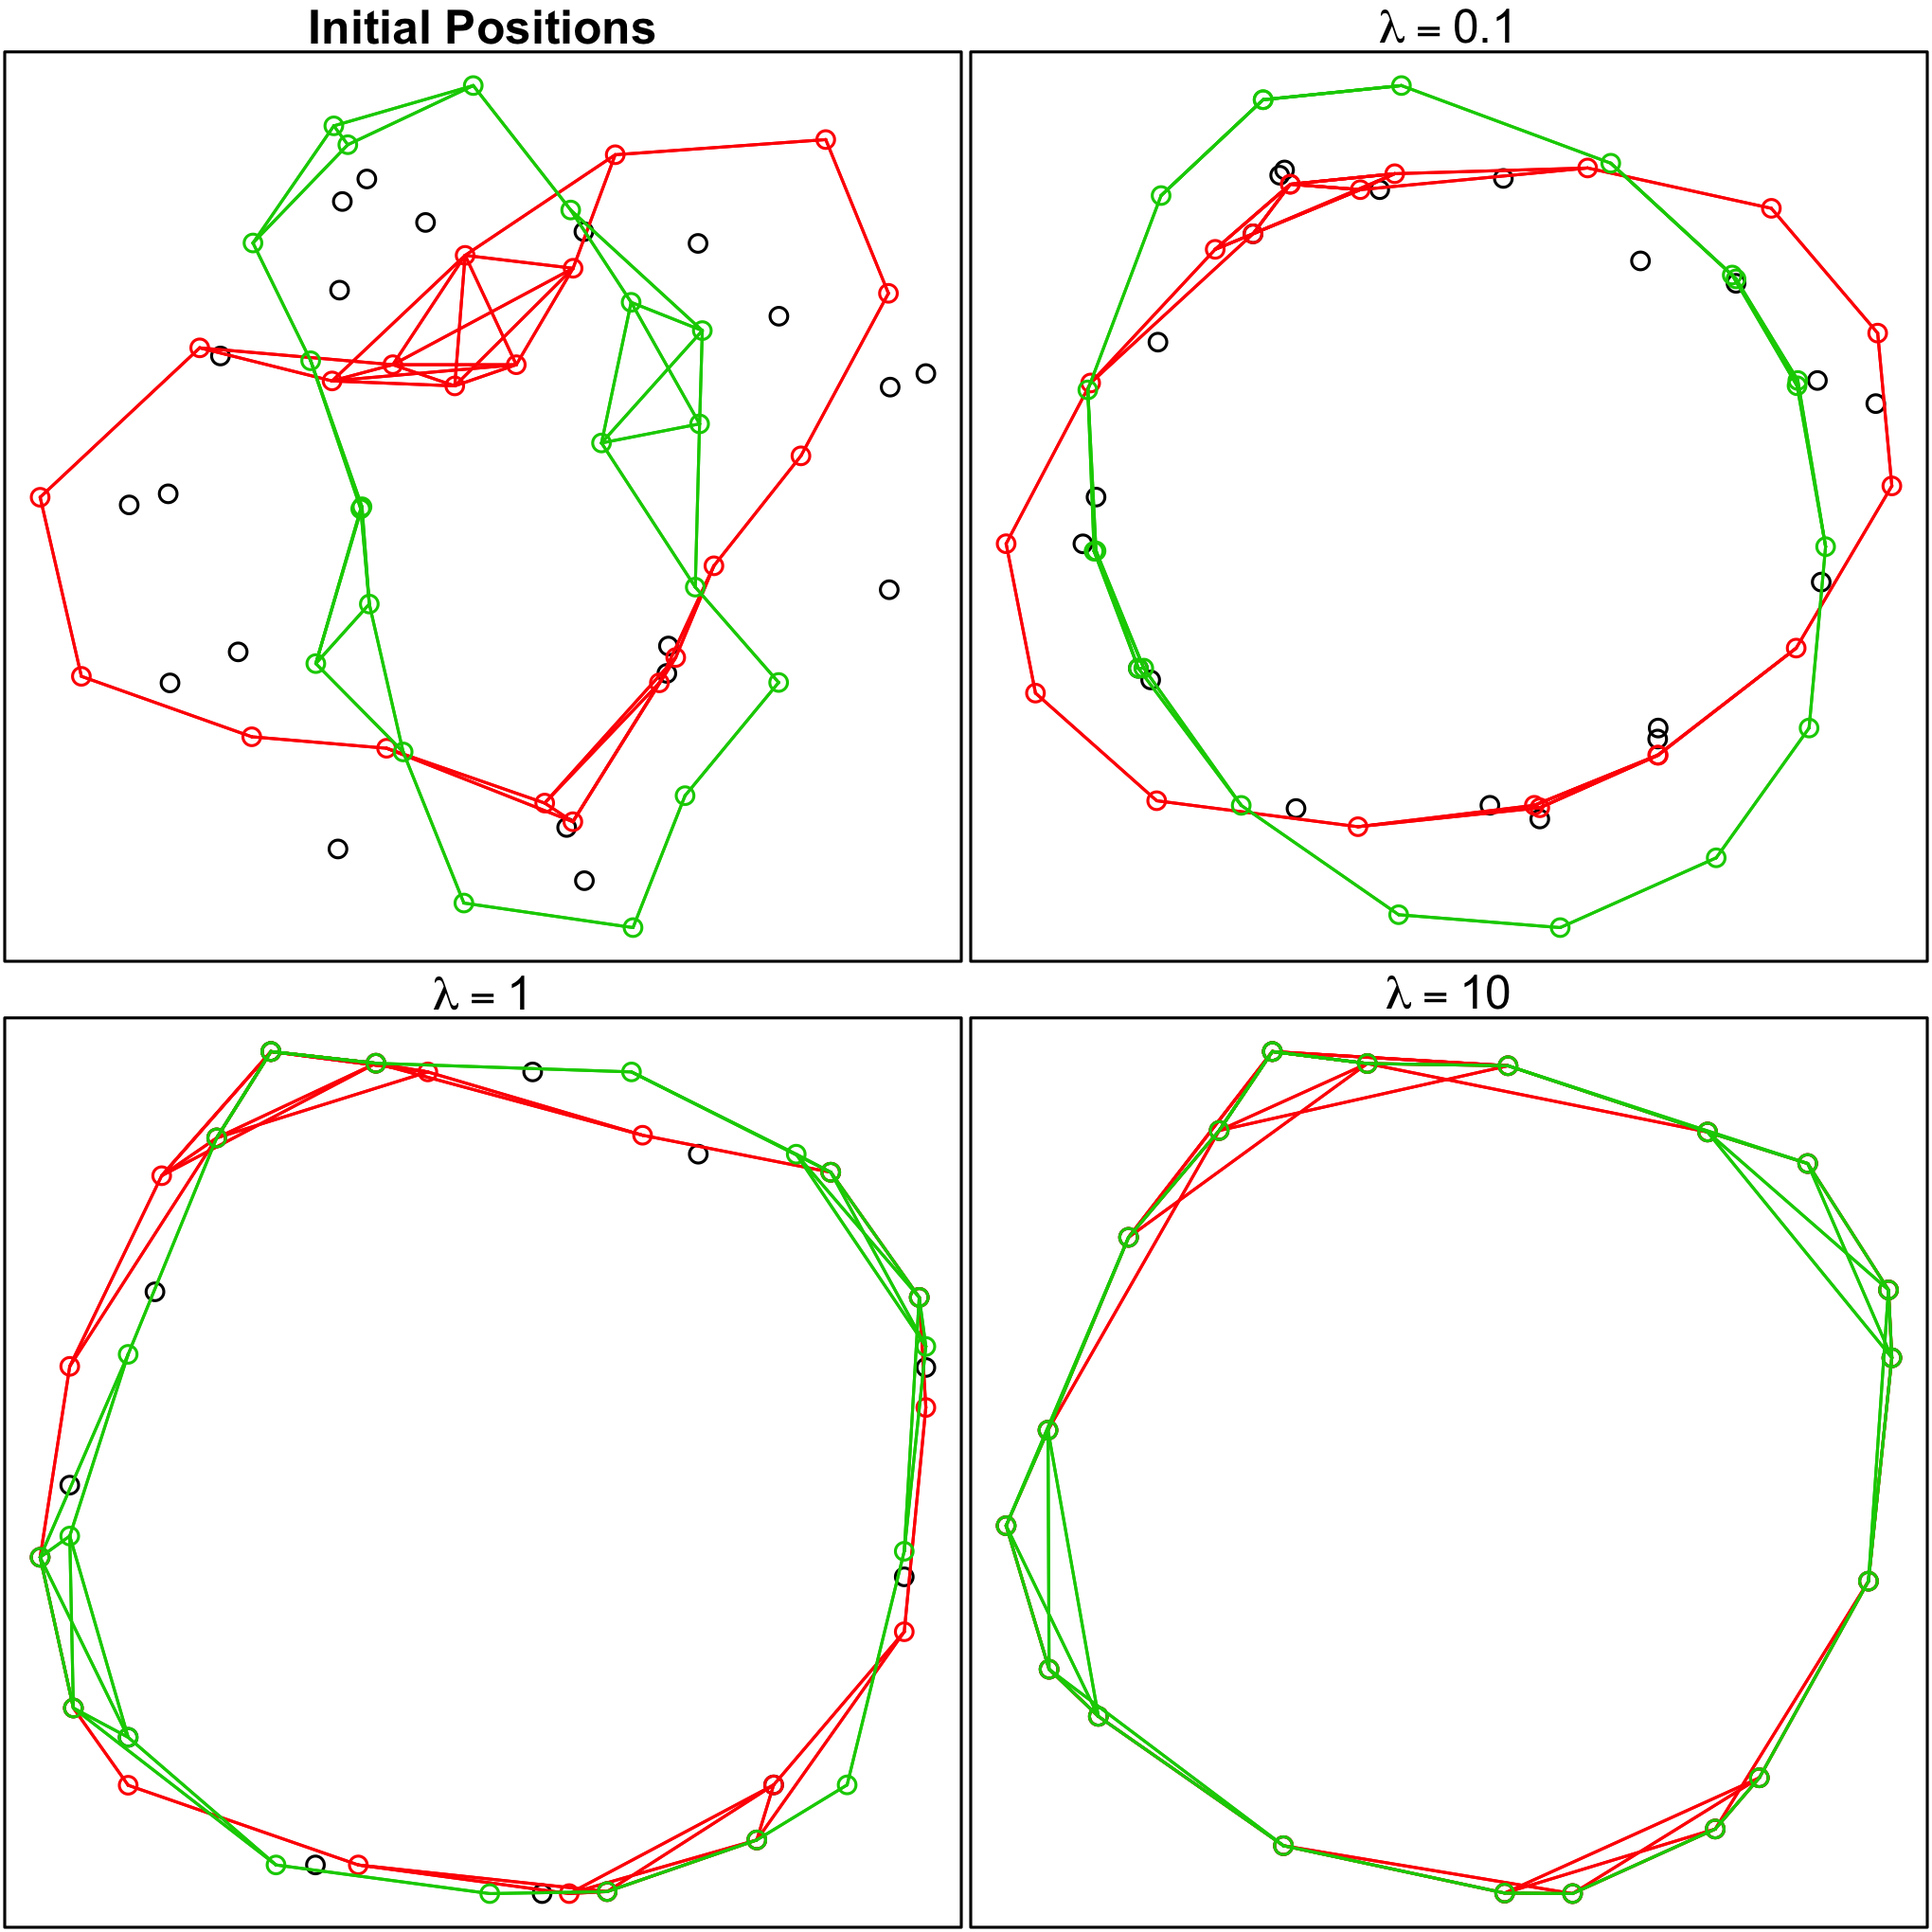
\includegraphics[width=0.4\textwidth]{plot_positions_individual} % requires the graphicx package
   \caption{Scatter plots showing the initial positions (top left plot) used in the optimization problem and the final ones for different values of $\lambda$ in the standard lasso approach. Black points represent the base positions $b_i$ and the red and green points (and lines) represent the two different layers of the graph. As the value of $\lambda$ increases deviations are more penalized and the optimal solution tends to be one where all layers collapse to a single graph.}
   \label{fig:pos_lasso}
\end{figure}
%
\begin{figure}[h!]
   \centering
   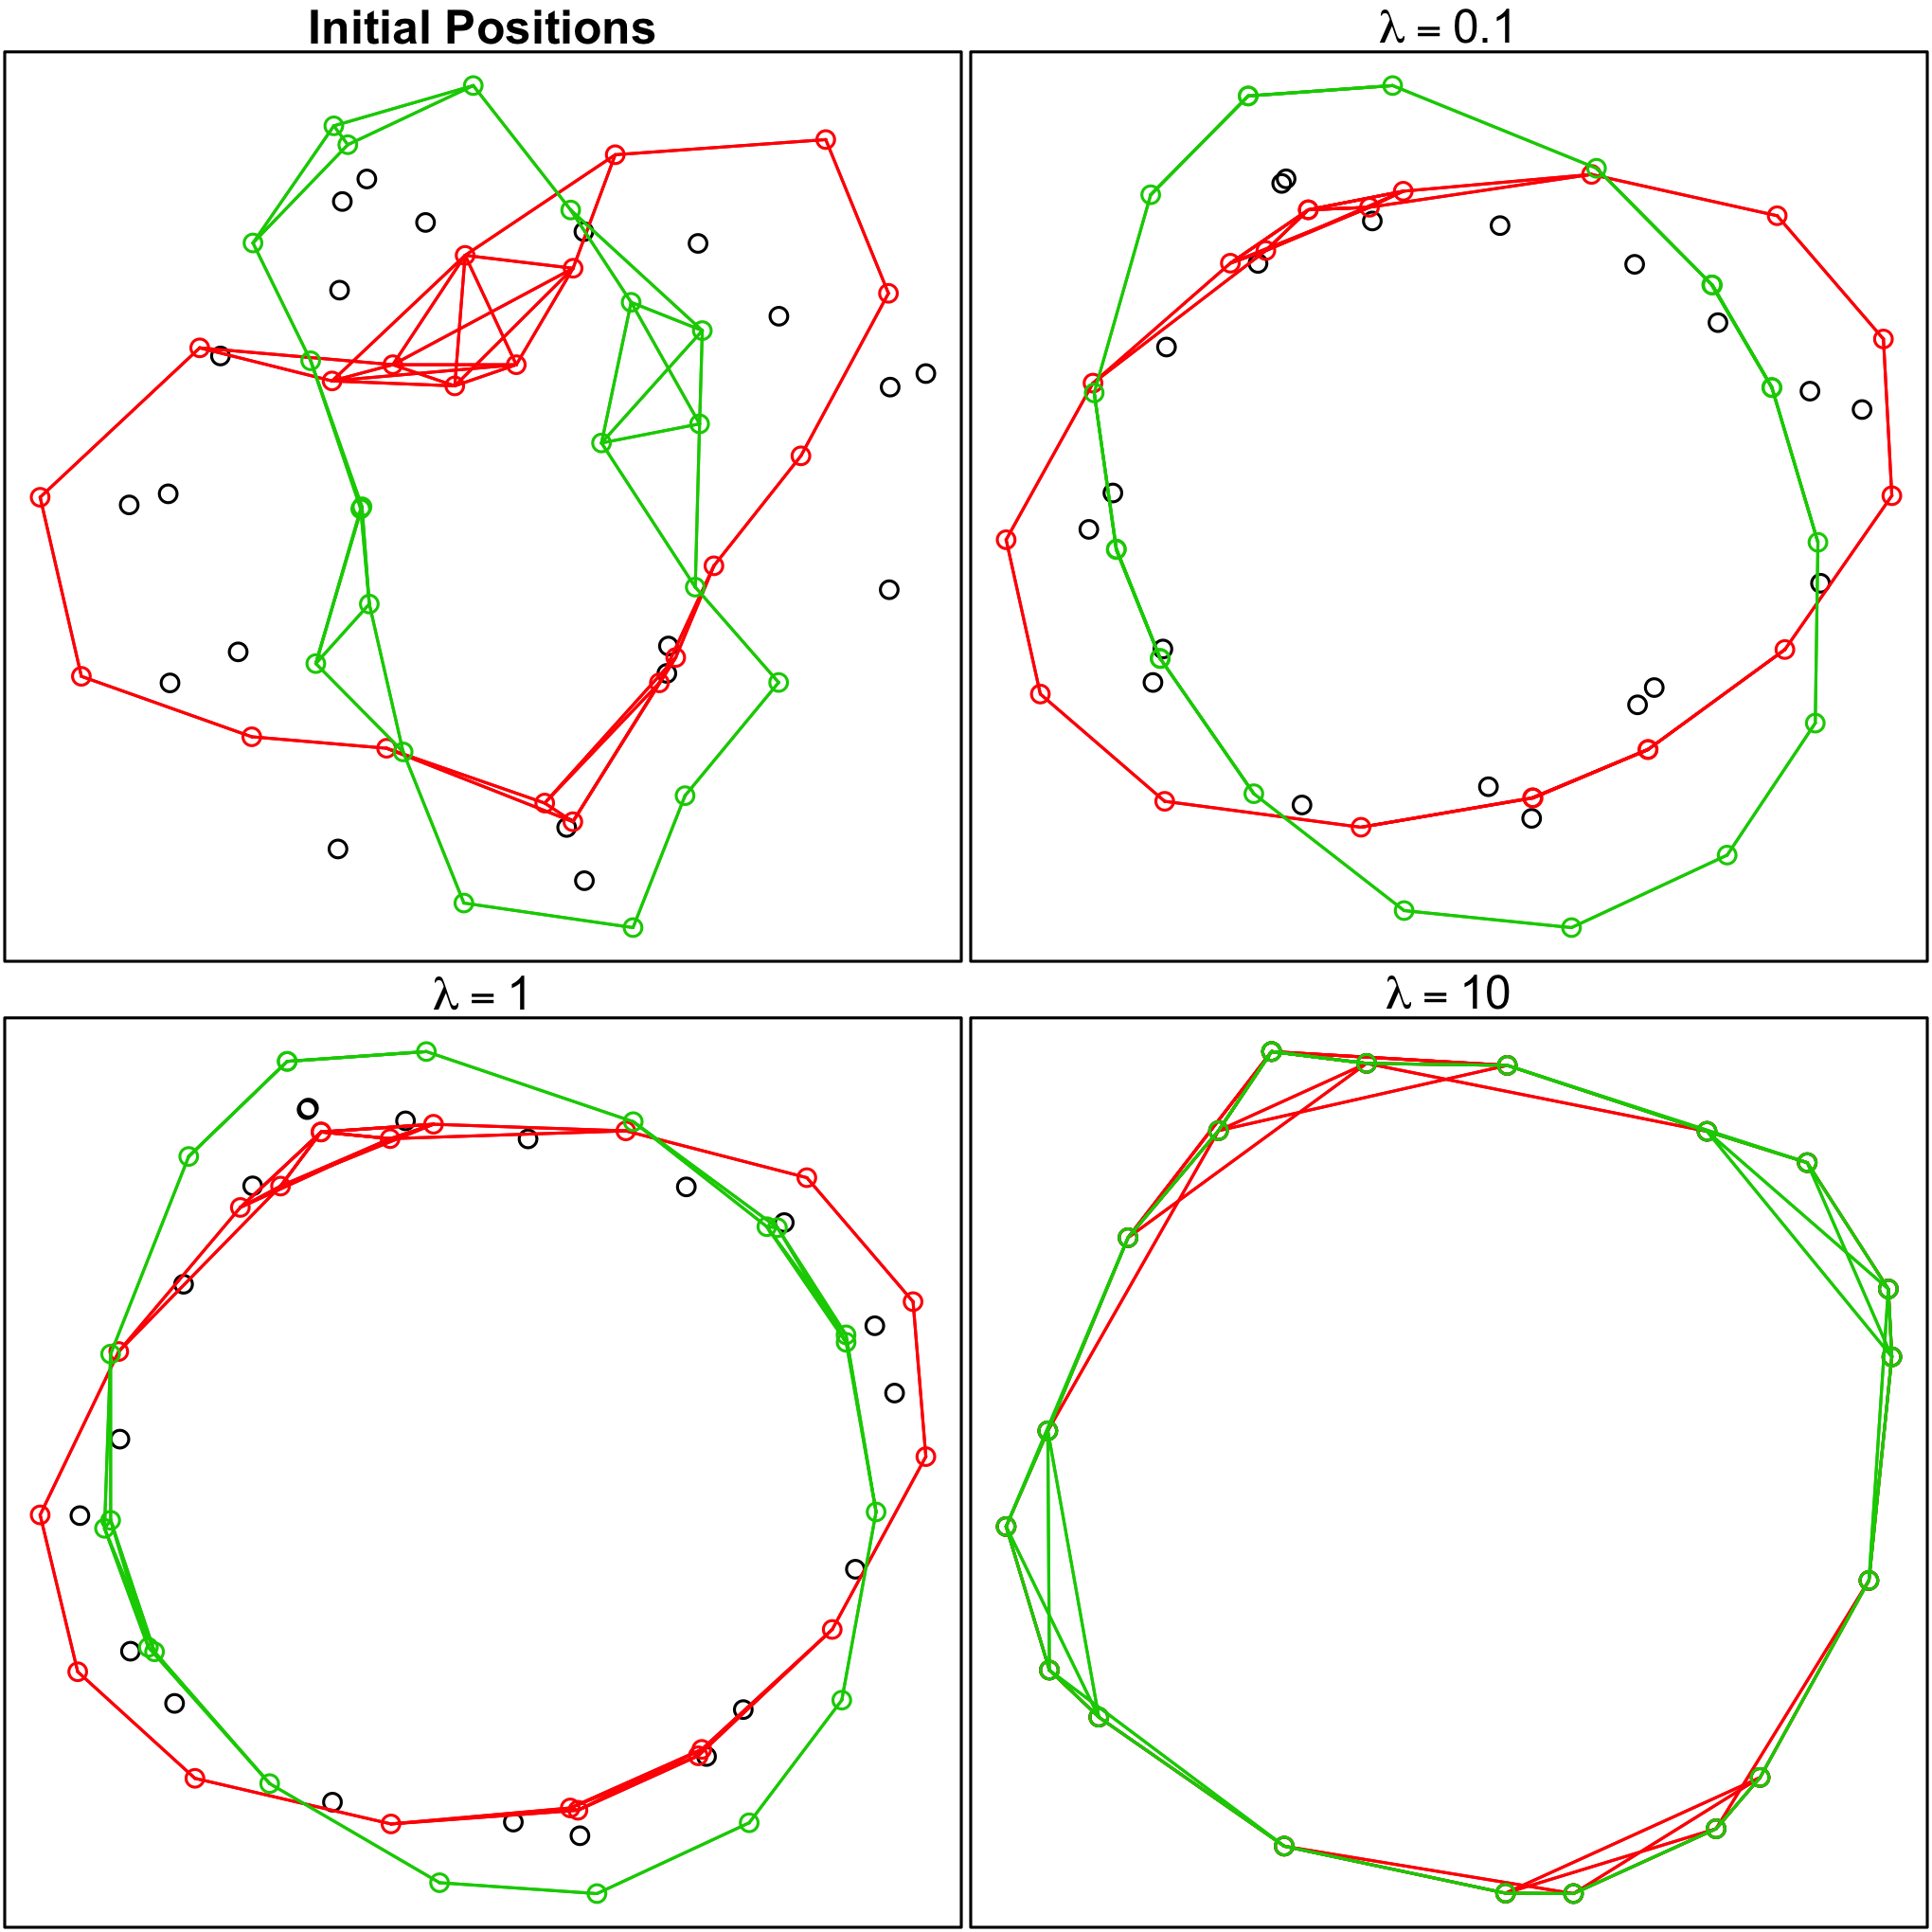
\includegraphics[width=0.4\textwidth]{plot_positions_group} % requires the graphicx package
   \caption{Scatter plots showing the initial positions (top left plot) used in the optimization problem and the final ones for different values of $\lambda$ in the group lasso approach. Black points represent the base positions $b_i$ and the red and green points (and lines) represent the two different layers of the graph. As the value of $\lambda$ increases deviations are more penalized and the optimal solution tends to be one where all layers collapse to a single graph. We can observe that for $\lambda=1$ the two layers are significantly more distinct than the ones in the standard lasso case.}
   \label{fig:pos_group}
\end{figure}

\begin{figure}[h!]
	\centering
	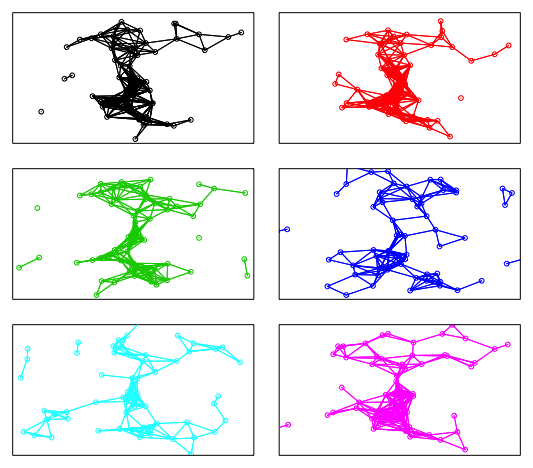
\includegraphics[width=0.6\textwidth]{six_gsa_graphs}
	\caption{A Real-World Network of Teachers in West Baltimore}
	\label{fig:gsa}
\end{figure}

In Figure \ref{fig:gsa}, we plot the results of our algorithm on a novel data set of teachers at a school in West Baltimore. As can be seen, the graphs are highly visually comparable, while also maintaining a substantial amount of expressiveness to demonstrate their individual structure. We believe this convincingly demonstrates the potential utility of our technique as a tool in social network analysis, as well as many other fields.

\section{Conclusion}

Despite not being a convex problem, a combination of convex methods and a good heuristic starting point have been shown to efficiently fit this novel class of models. In addition, they have demonstrated all of the properties for which they were intended, and several others additionally. As demonstrated, HLSMs are capable of producing comparable graph layouts for the layers of a multigraph, and are also capable of performing layer-wise dimensionality reduction in order to meaningfully simplify this complex form of data.

HLSMs are also valuable for refining the layouts determined by current Latent Space Model implementations, as can been seen in the differences between the initializations, and the final estimates. While it is possible that many likelihoods accurately ``represent'' the graph (meaning essentially that their classification accuracy for edges is high \cite{Hoff2002}) , this further convex optimization is valuable in finding solutions that are meaningful to human interpreters. Furthermore, our fitting procedure was found to converge to a good solution far faster than the HMC implementation with which we compared it.

Having demonstrated the basic feasibility, effectiveness, and utility, of HLSMs, the next steps will be to push its limits on different kinds of graphs, and different numbers of layers. Several different guests at our poster session mentioned additional problems, including in medical domains, and the interpretability of deep neural nets, to which our method might be able to contribute. We look forward to exploring these additional problem spaces.
\clearpage


\textbf{NEXT:}
\section{Comparing Fitting Methods}
Because why not (not crucial, but maybe important since it's a convex method for a non-convex problem)
\subsection{Stan/HMC}
The way LSMs are fit now -- appear to be way slower, and worse
\subsection{Coordinate-Wise Optimization}
A cute idea, but one that I haven't gotten to work yet. If it comes through.

\section{Visual Comparability Tests}
The most important, and the most subjective. Anecdotal results above were strong though, maybe clear enough to be easy. The comparison, in every case, will be with sets of independently fit LSMs. Which though, already, given the two ovals model, we've beaten substantially, in terms of polish at least.

\section{Dimensionality Reduction Tests}
Create graphs of different degrees of correlation -- what's the rxp between lambda, rho, and layer=0?

\section{Comparability and Accuracy}
What happens to the accuracy when you force a set of dissimilar graphs to be similar in latent position?

\section{A Real-World Test Case}
My school data, where background knowledge of the system allows validity checks for the produced layouts
\subsection{Grade Clusters}
Do the forced-similar graphs preserve grade clusters?
\subsection{Subject Clusters}
Same, for math/science/lit clusters
\subsection{Role Clusters}
Same, for teacher/admin/staff clusters

Else? Maybe a demonstration with another data set, like Samson? Would be cool to say something new about something so canonical.



\clearpage

\bibliography{sample.bib}

\section*{Appendix: Link to R scripts}

The proximal descent methods described in this report were implemented using the R language. All scripts are available in the following git hub repository: \url{https://github.com/amloewi/hlsm}. The main R script is located at \url{https://github.com/amloewi/hlsm/blob/master/R/final_project.R}

\end{document}
